\begin{center}

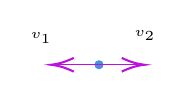
\begin{tikzpicture}[x=0.75pt,y=0.75pt,yscale=-1,xscale=1]
%uncomment if require: \path (0,300); %set diagram left start at 0, and has height of 300

%Shape: Circle [id:dp8577753533756336] 
\draw  [color={rgb, 255:red, 74; green, 144; blue, 226 }  ,draw opacity=1 ][fill={rgb, 255:red, 74; green, 144; blue, 226 }  ,fill opacity=1 ] (196.17,140) .. controls (196.17,138.94) and (197.03,138.09) .. (198.09,138.09) .. controls (199.14,138.09) and (200,138.94) .. (200,140) .. controls (200,141.06) and (199.14,141.91) .. (198.09,141.91) .. controls (197.03,141.91) and (196.17,141.06) .. (196.17,140) -- cycle ;
%Straight Lines [id:da03072071750773664] 
\draw [color={rgb, 255:red, 189; green, 16; blue, 224 }  ,draw opacity=1 ]   (198.09,140) -- (177,140) ;
\draw [shift={(175,140)}, rotate = 360] [color={rgb, 255:red, 189; green, 16; blue, 224 }  ,draw opacity=1 ][line width=0.75]    (10.93,-3.29) .. controls (6.95,-1.4) and (3.31,-0.3) .. (0,0) .. controls (3.31,0.3) and (6.95,1.4) .. (10.93,3.29)   ;
%Straight Lines [id:da26303253715785346] 
\draw [color={rgb, 255:red, 189; green, 16; blue, 224 }  ,draw opacity=1 ]   (198.09,140) -- (218,140) ;
\draw [shift={(220,140)}, rotate = 180] [color={rgb, 255:red, 189; green, 16; blue, 224 }  ,draw opacity=1 ][line width=0.75]    (10.93,-3.29) .. controls (6.95,-1.4) and (3.31,-0.3) .. (0,0) .. controls (3.31,0.3) and (6.95,1.4) .. (10.93,3.29)   ;

% Text Node
\draw (164,123.4) node [anchor=north west][inner sep=0.75pt]  [font=\tiny]  {$v_{1}$};
% Text Node
\draw (214,122.4) node [anchor=north west][inner sep=0.75pt]  [font=\tiny]  {$v_{2}$};


\end{tikzpicture}

\end{center}